\chapter*{Lima\markboth{Lima}{}}
\section*{5 juin 2015}
De Cusco à Lima, trajet en bus de luxe avec repas, films et sièges confortables on se croirait en avion. 

\begin{center} 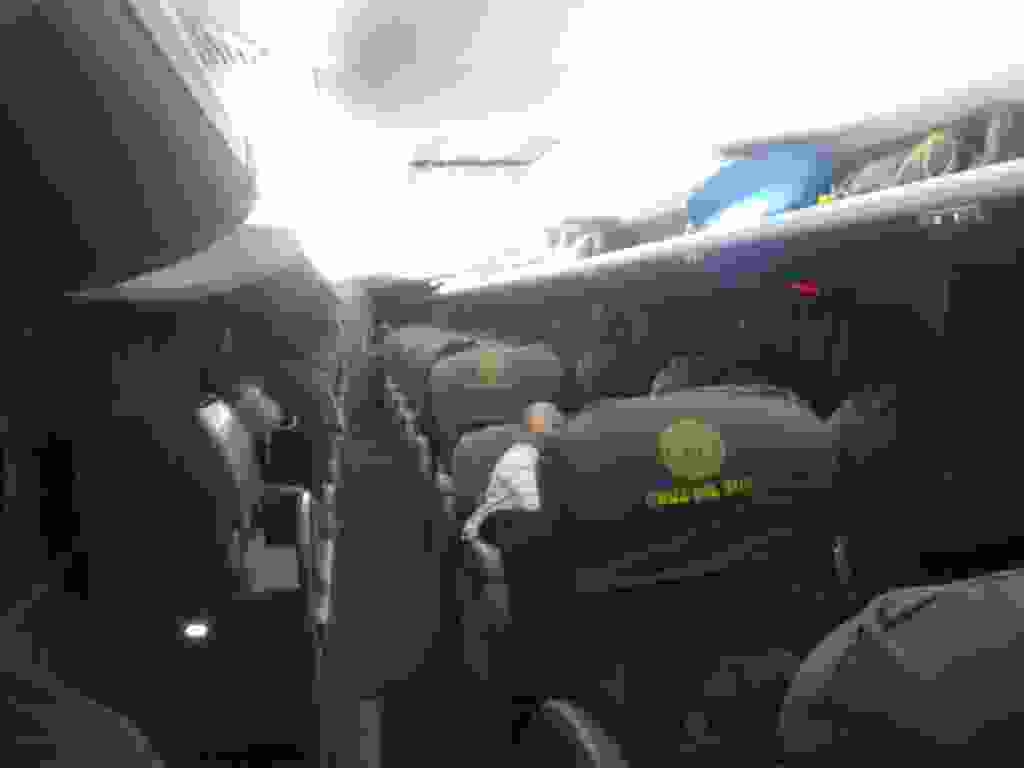
\includegraphics[width=\mywidth]{../wp-content/uploads/2015/06/P5304567-1024x768.jpg} \end{center}
\vspace{-\topsep}
\vspace{-5mm}
\pagebreak

J'ai visité Lima en vélo : la ville est immense et le trafic énorme mais heureusement il y a quelques belles pistes cyclables sur les grandes avenues. 

\begin{center} 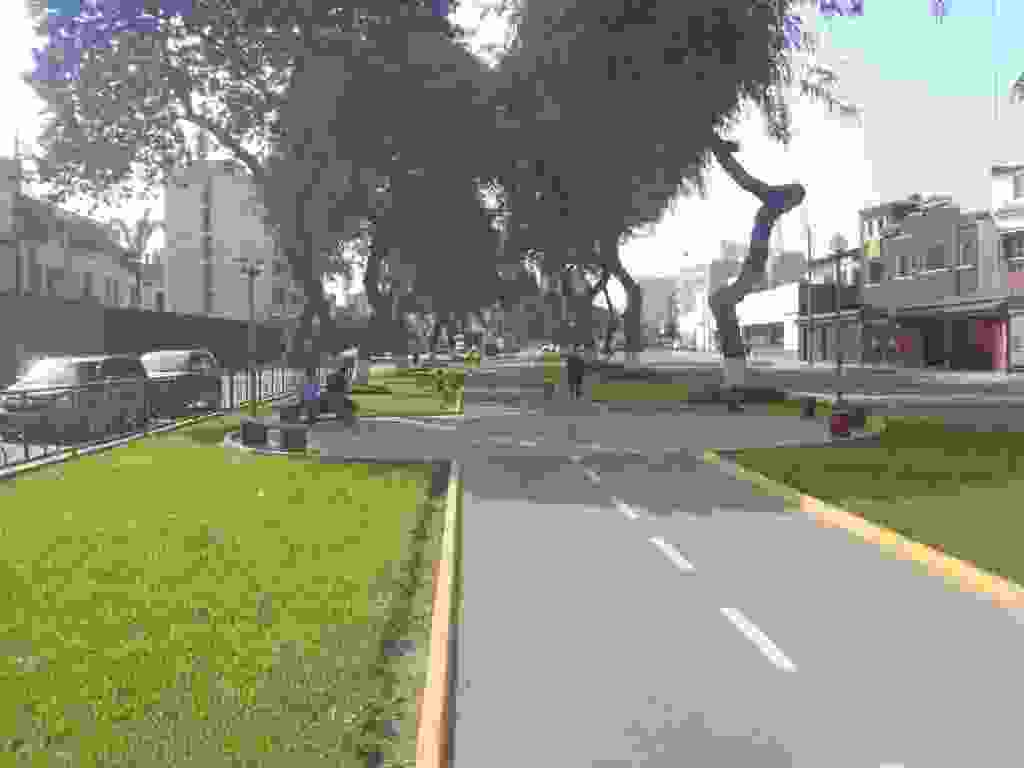
\includegraphics[width=\mywidth]{../wp-content/uploads/2015/06/P5314573-1024x768.jpg} \end{center}

\begin{center} 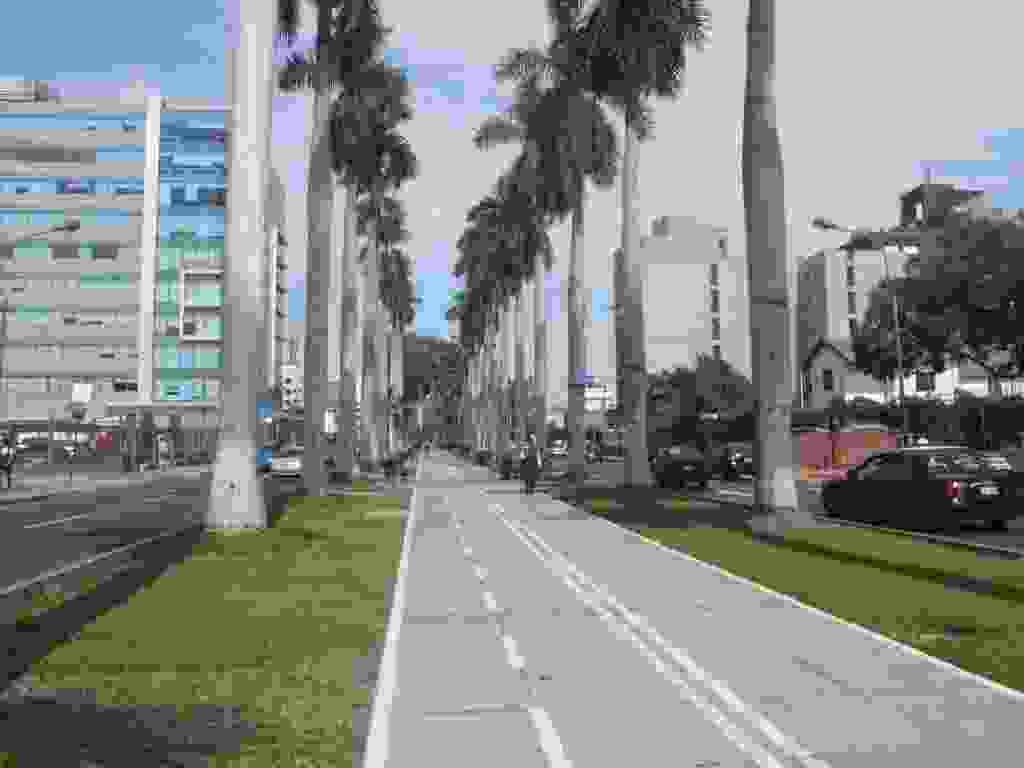
\includegraphics[width=\mywidth]{../wp-content/uploads/2015/06/P6014590-1024x768.jpg} \end{center}
\vspace{-\topsep}
\vspace{-2.25mm}
 \pagebreak

Le centre de Lima :  La Plaza San Martin.

\begin{center} 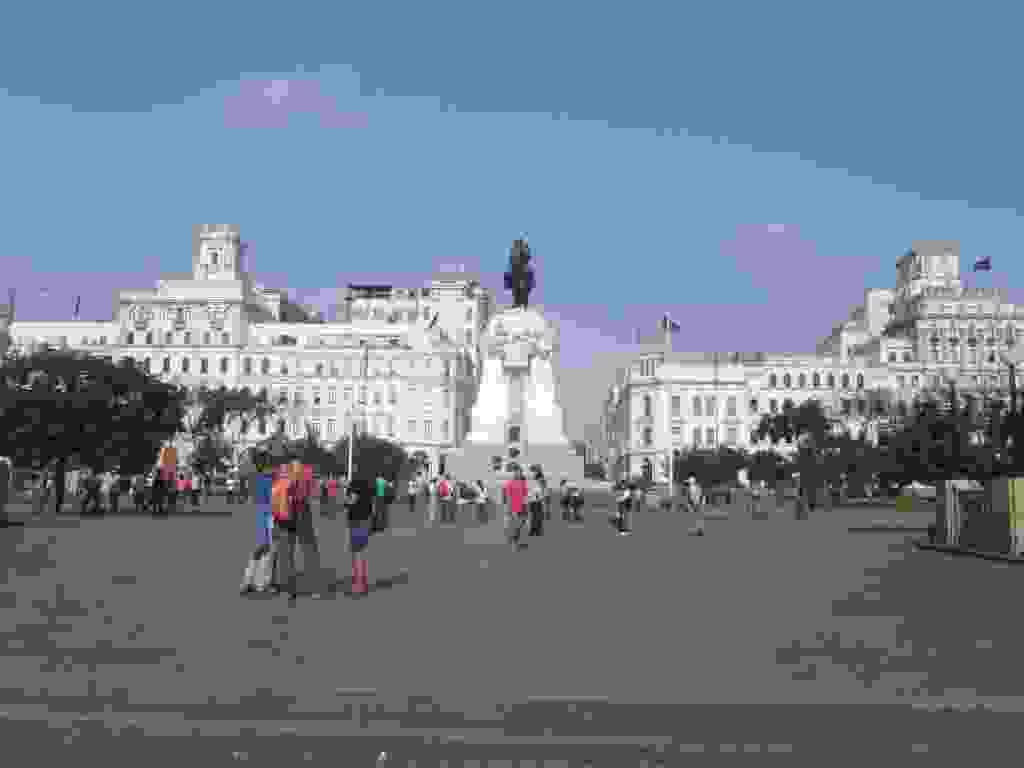
\includegraphics[width=\mywidth]{../wp-content/uploads/2015/06/P5314578-1024x768.jpg} \end{center}

\begin{center} 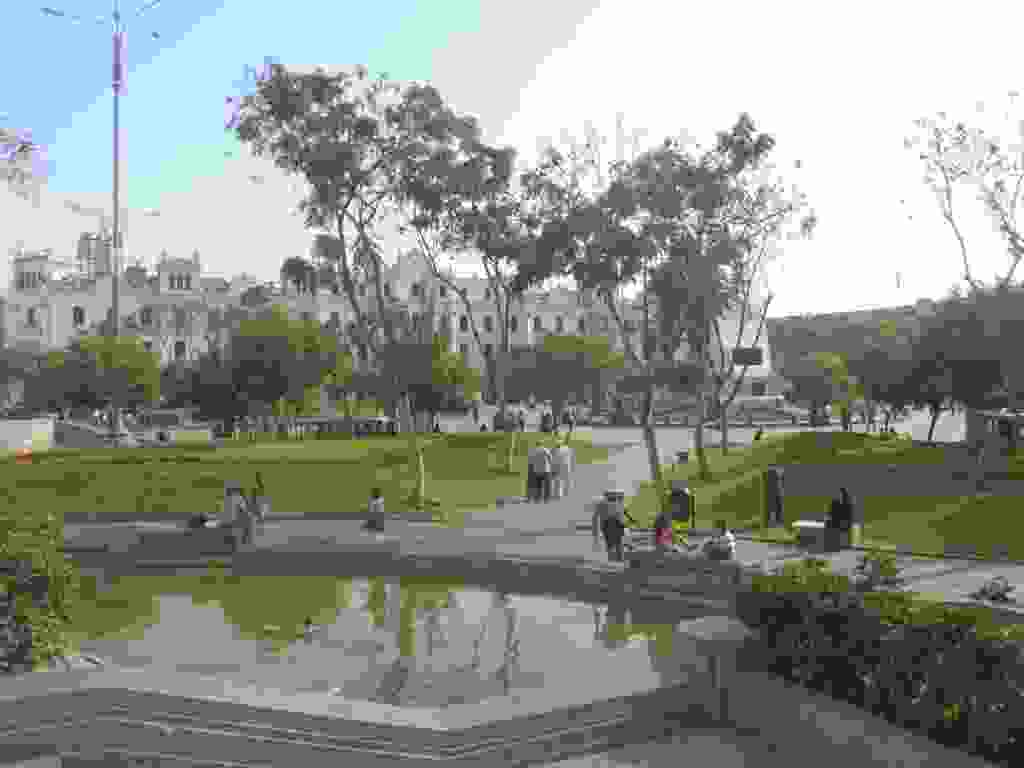
\includegraphics[width=\mywidth]{../wp-content/uploads/2015/06/P5314579-1024x768.jpg} \end{center}
 \vspace{-\topsep}
 \vspace{-3.25mm}
\pagebreak

La Plaza de Armas avec la cathédrale et le palais gouvernemental.

\begin{center} 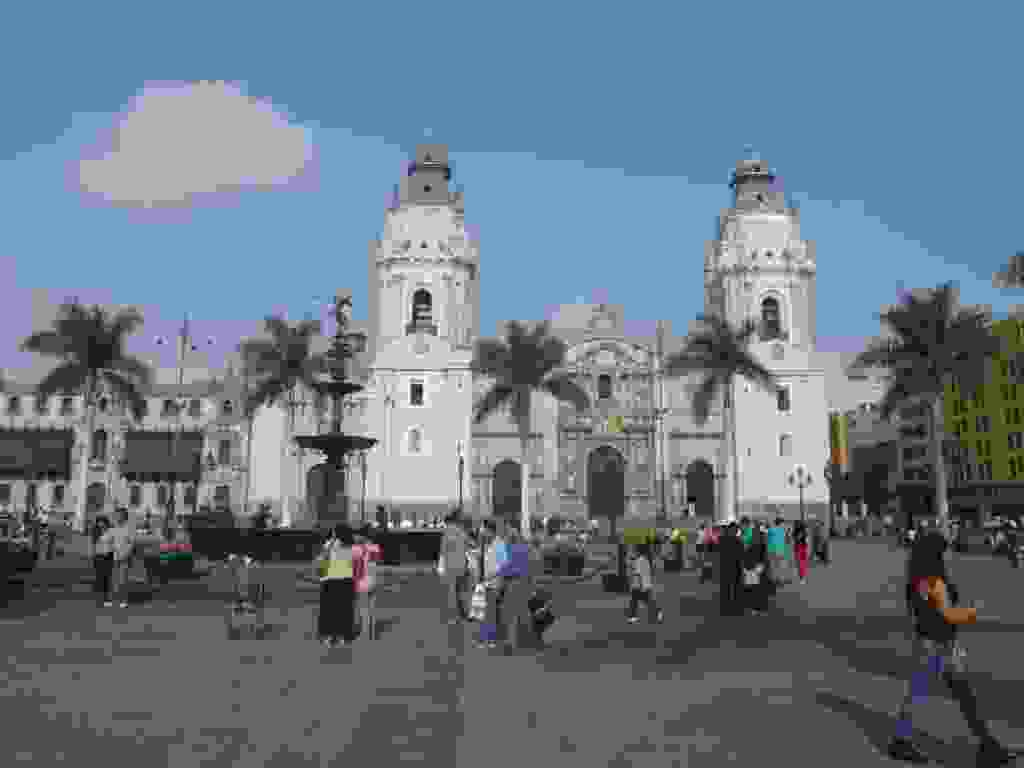
\includegraphics[width=\mywidth]{../wp-content/uploads/2015/06/P5314582-1024x768.jpg} \end{center}

\begin{center} 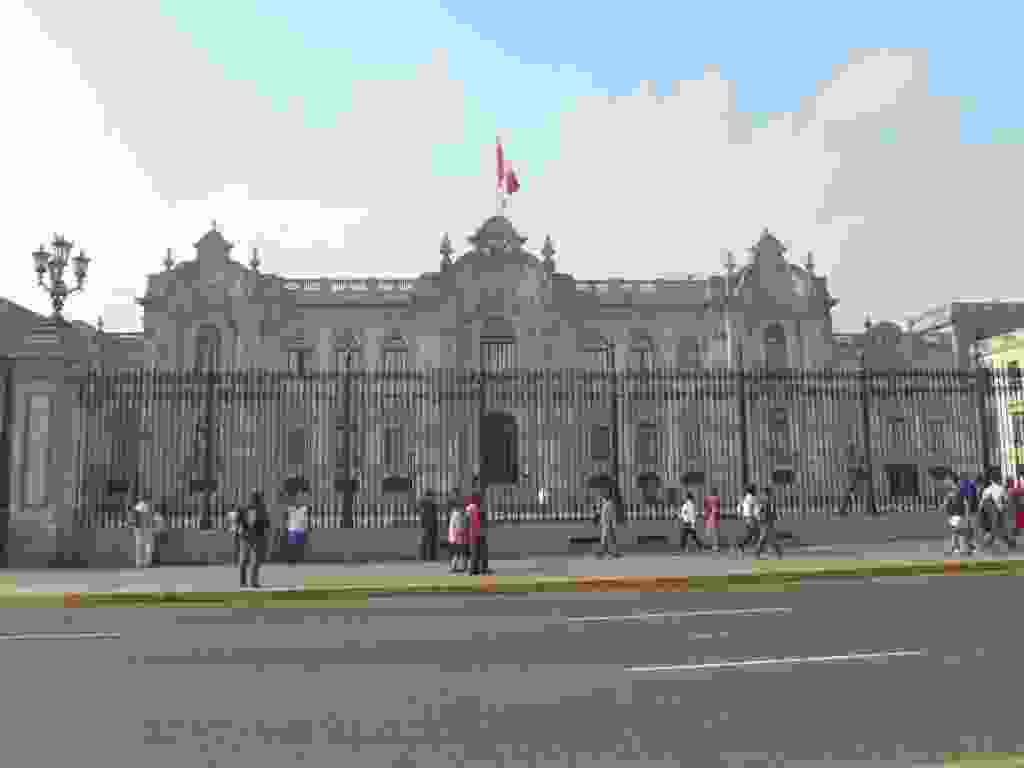
\includegraphics[width=\mywidth]{../wp-content/uploads/2015/06/P5314585-1024x768.jpg} \end{center}
\vspace{-\topsep}
\vspace{-3.25mm}
 \pagebreak

L'église San Francisco que j'ai visitée : avec notamment une belle bibliotheque et les catacombes où des dizaines de milliers de personnes ont été enterrées. Dommage les photos étaient interdites a l'intérieur. 

\begin{center} 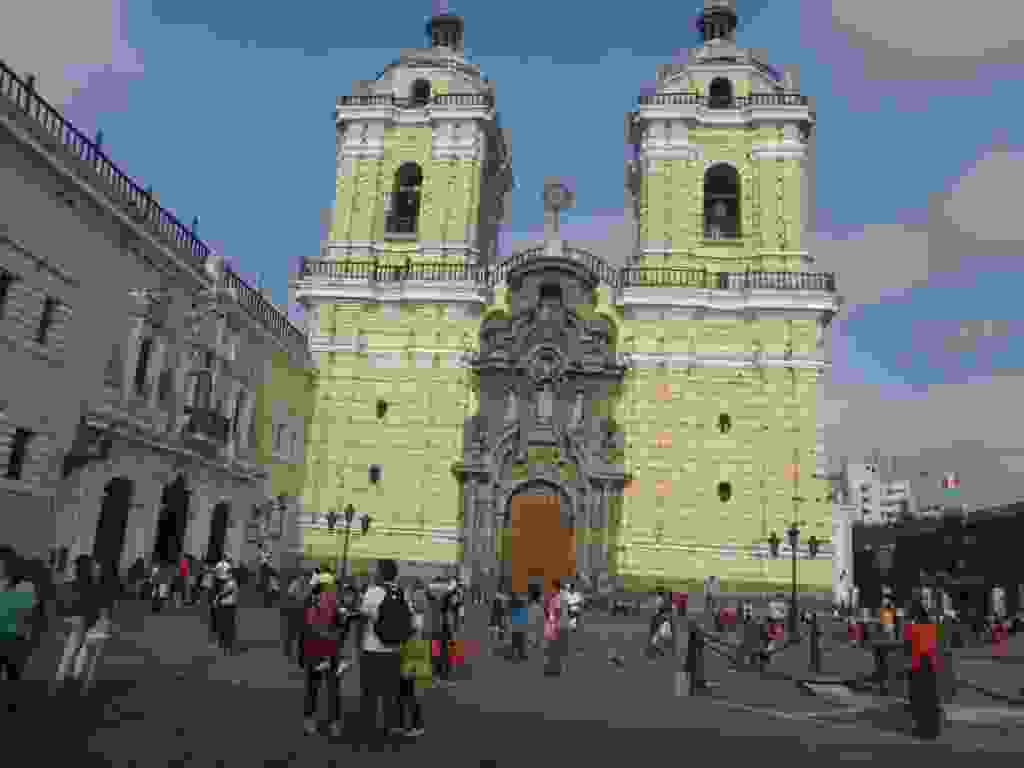
\includegraphics[width=\mywidth]{../wp-content/uploads/2015/06/P5314586-1024x768.jpg} \end{center}

Le quartier Miraflores au sud de Lima : quartier touristique et aisé au bord de l'océan Pacifique. 

\begin{center} 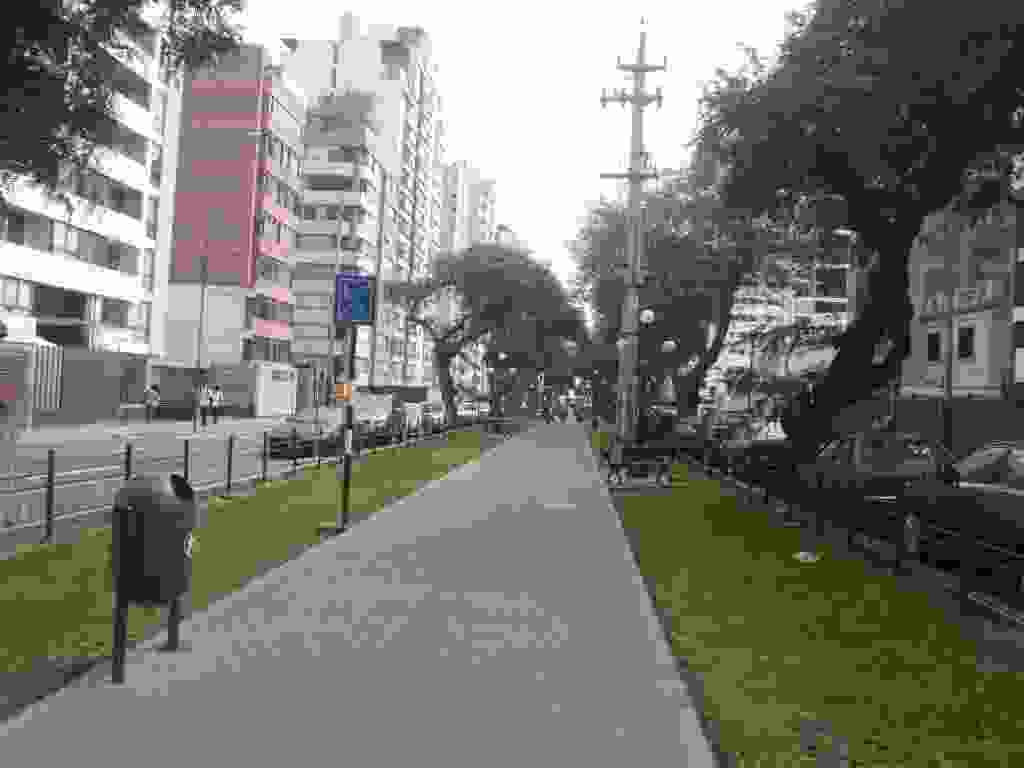
\includegraphics[width=\mywidth]{../wp-content/uploads/2015/06/P60145911-1024x768.jpg} \end{center}
\vspace{-\topsep}
\vspace{-0.75mm}
\pagebreak
~\\~\\
\begin{center} 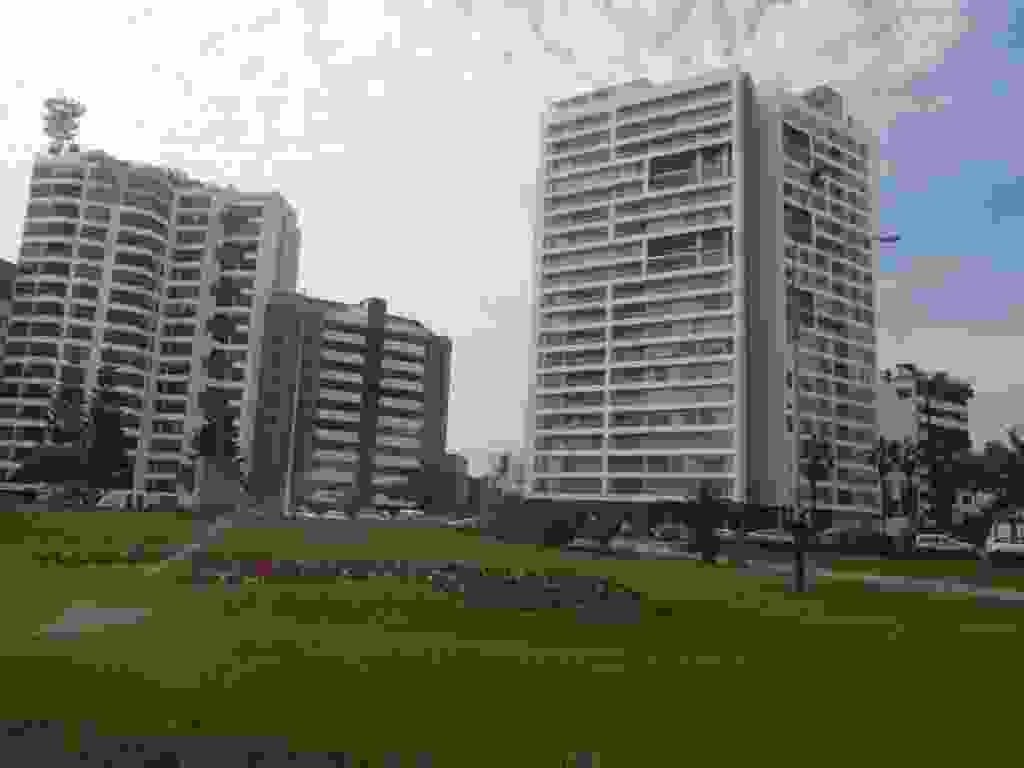
\includegraphics[width=\mywidth]{../wp-content/uploads/2015/06/P6014593-1024x768.jpg} \end{center}
~\\
\begin{center} 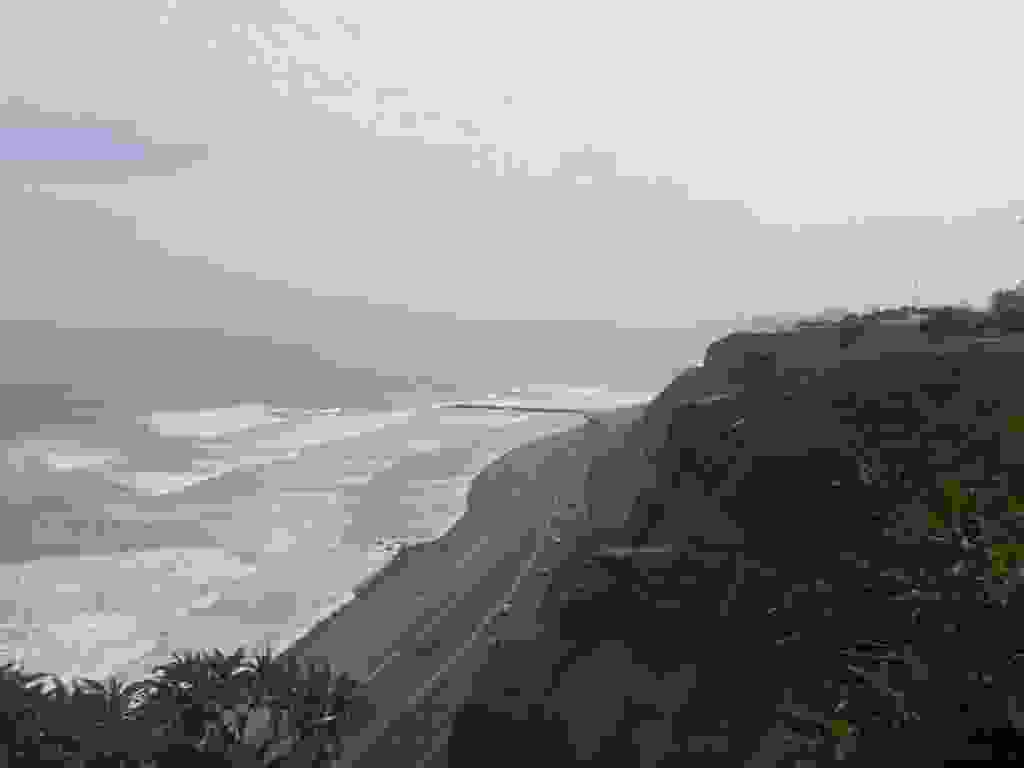
\includegraphics[width=\mywidth]{../wp-content/uploads/2015/06/P6014595-1024x768.jpg} \end{center}

\begin{center} 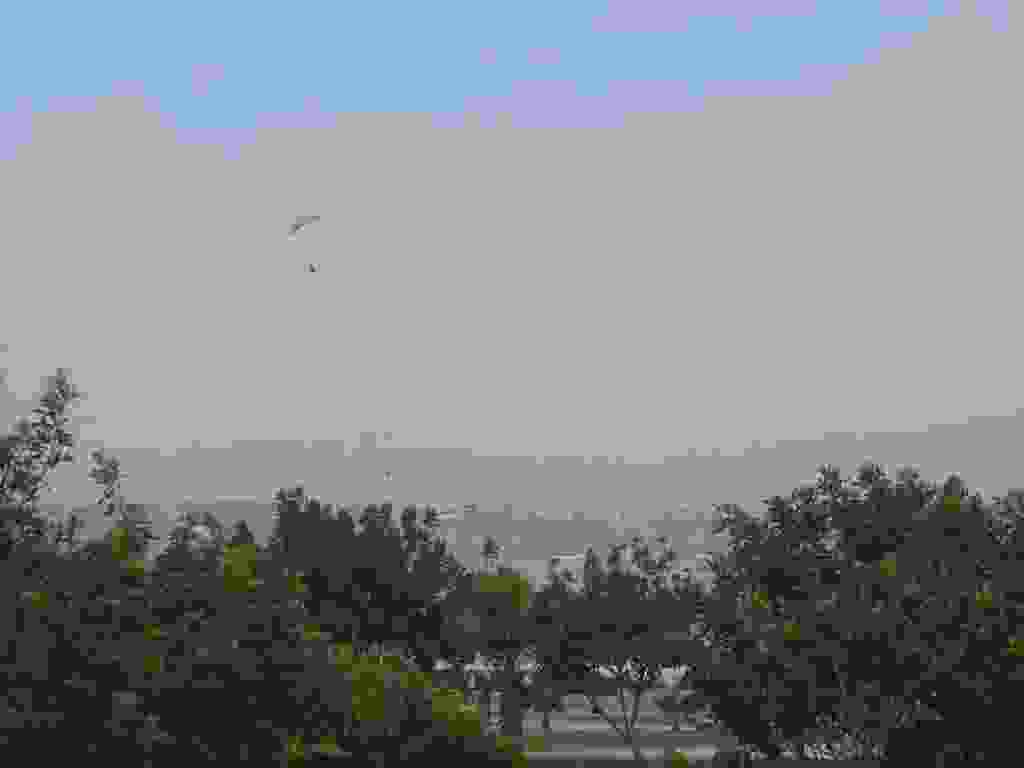
\includegraphics[width=\mywidth]{../wp-content/uploads/2015/06/P6014597-1024x768.jpg} \end{center}

\begin{center} 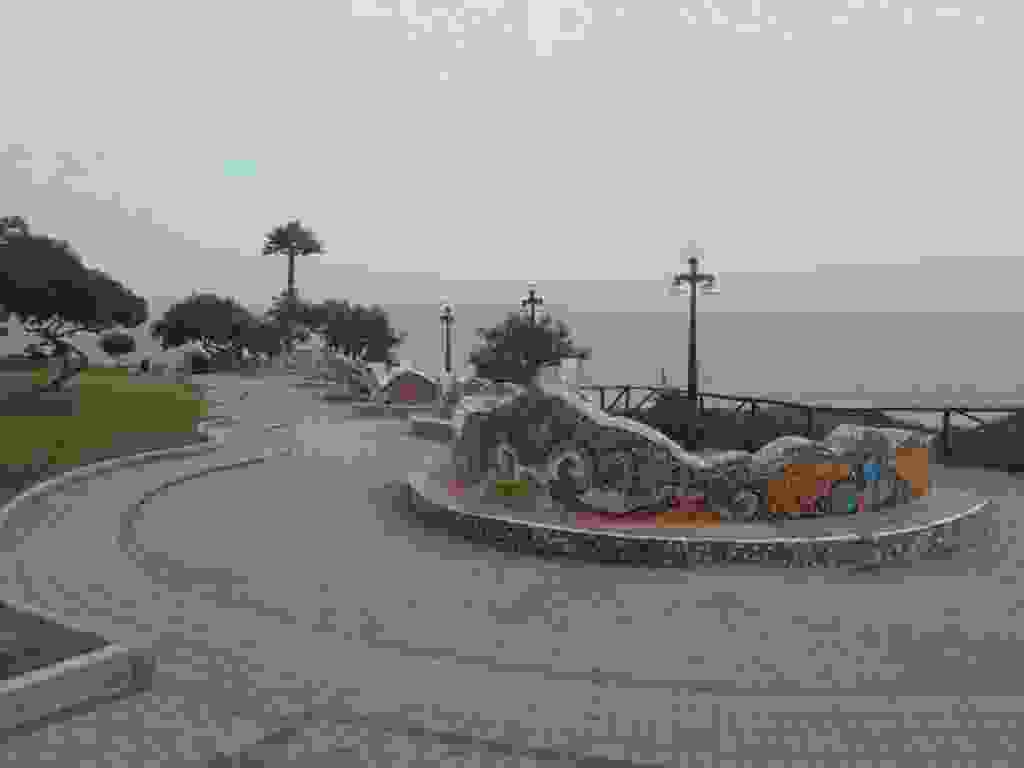
\includegraphics[width=\mywidth]{../wp-content/uploads/2015/06/P6014599-1024x768.jpg} \end{center}

\begin{center} 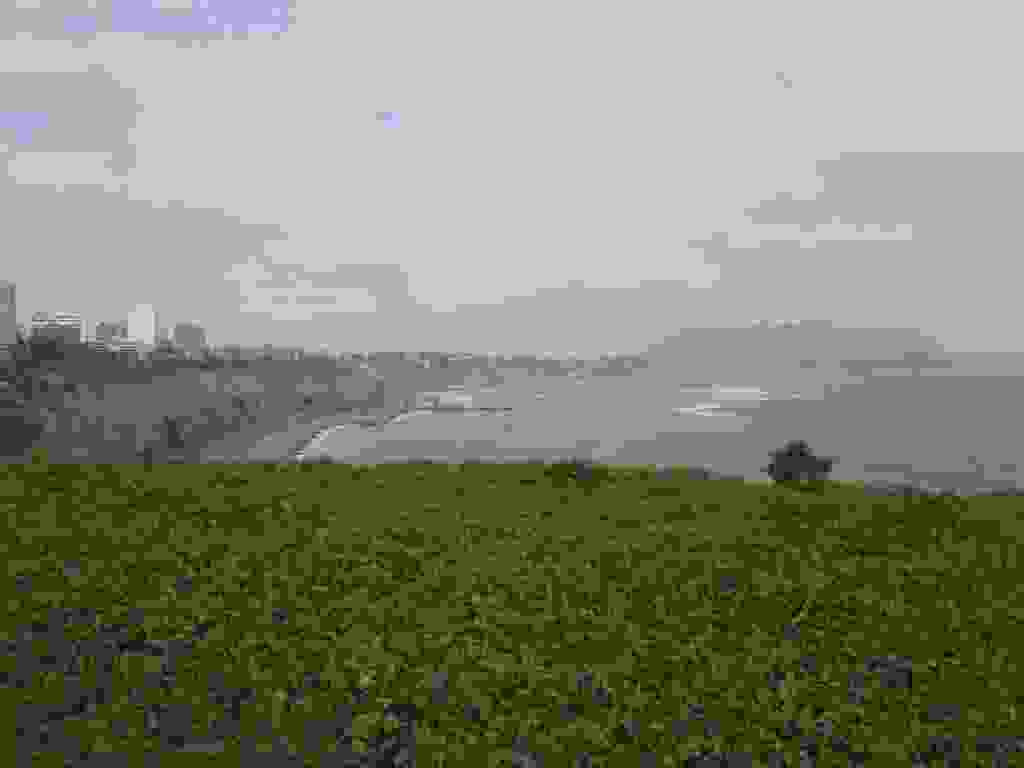
\includegraphics[width=\mywidth]{../wp-content/uploads/2015/06/P6014600-1024x768.jpg} \end{center}

On y trouve de bons ceviches, \og la \fg\ spécialité péruvienne de poisson et fruits de mer marinés. 

\begin{center} 
\includegraphics[width=\mywidth]{../wp-content/uploads/2015/06/P6014602-1024x768.jpg} \end{center}
 \vspace{-\topsep}
 \vspace{-3.25mm}
\pagebreak

Le quartier Barranco encore plus au sud : le quartier bohème de Lima. 

\begin{center} 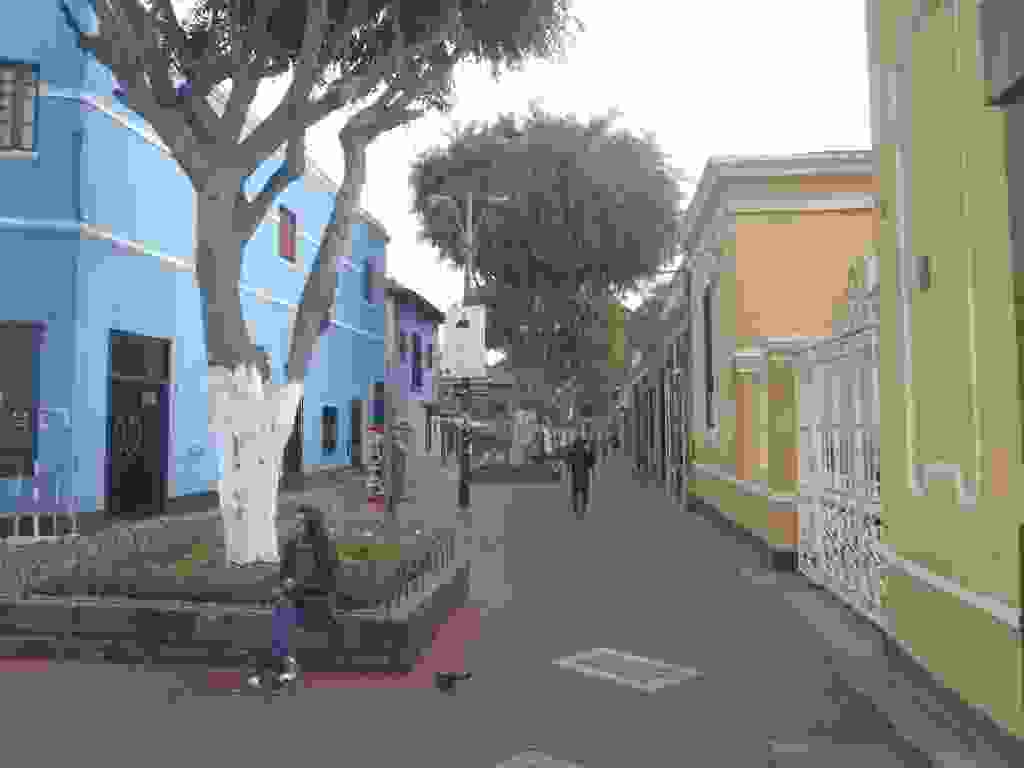
\includegraphics[width=\mywidth]{../wp-content/uploads/2015/06/P6014607-1024x768.jpg} \end{center}
~\\~\\
\begin{center} 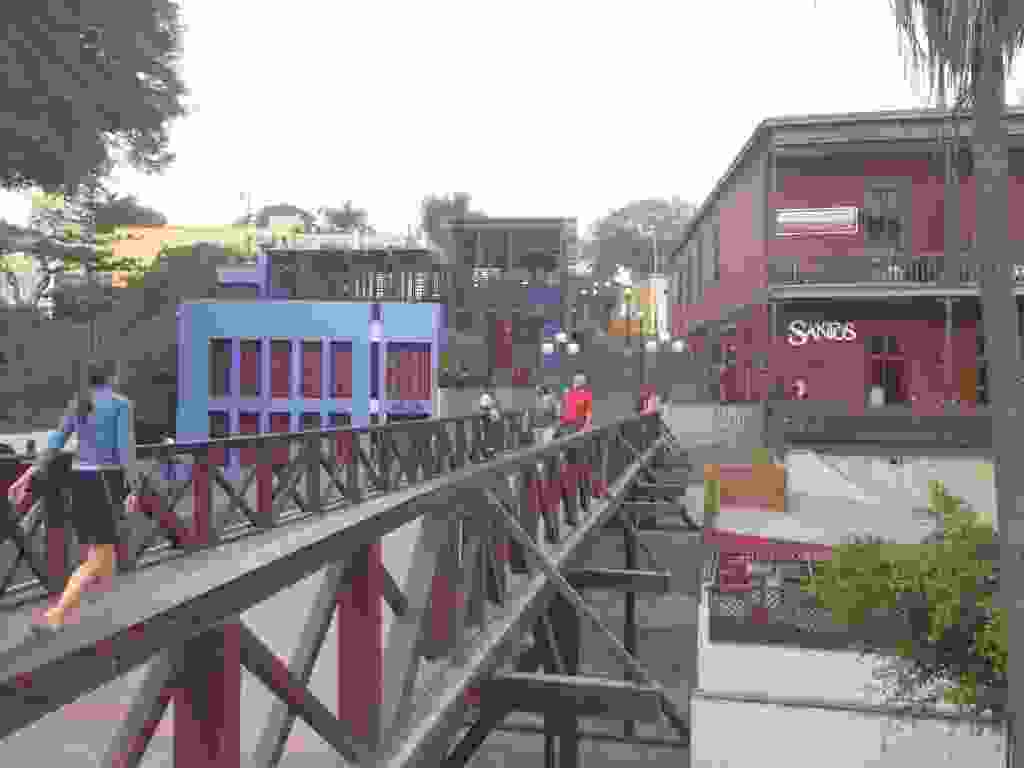
\includegraphics[width=\mywidth]{../wp-content/uploads/2015/06/P6014605-1024x768.jpg} \end{center}
\vspace{-\topsep}
\pagebreak
~
\begin{center} 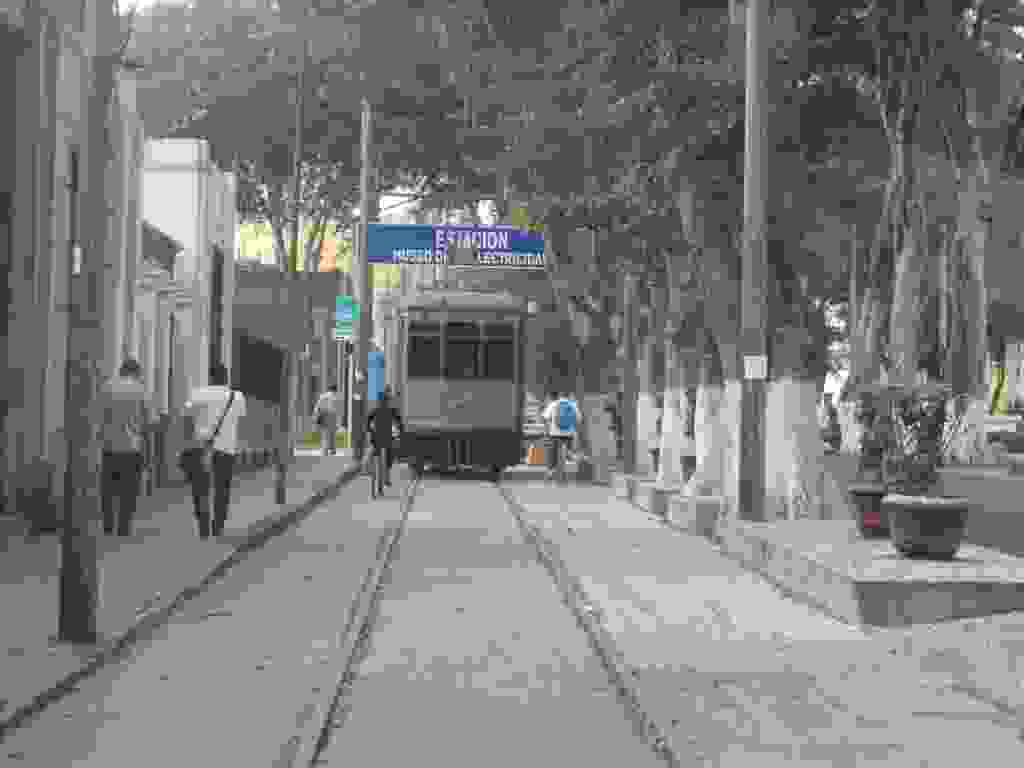
\includegraphics[width=\mywidth]{../wp-content/uploads/2015/06/P6014606-1024x768.jpg} \end{center}

Enfin la petite pépite de Lima, le parc de la Reserva et son circuit des fontaines magiques : un parcours de 13 fontaines avec musique synchronisée aux jets d'eau. 

\begin{center} 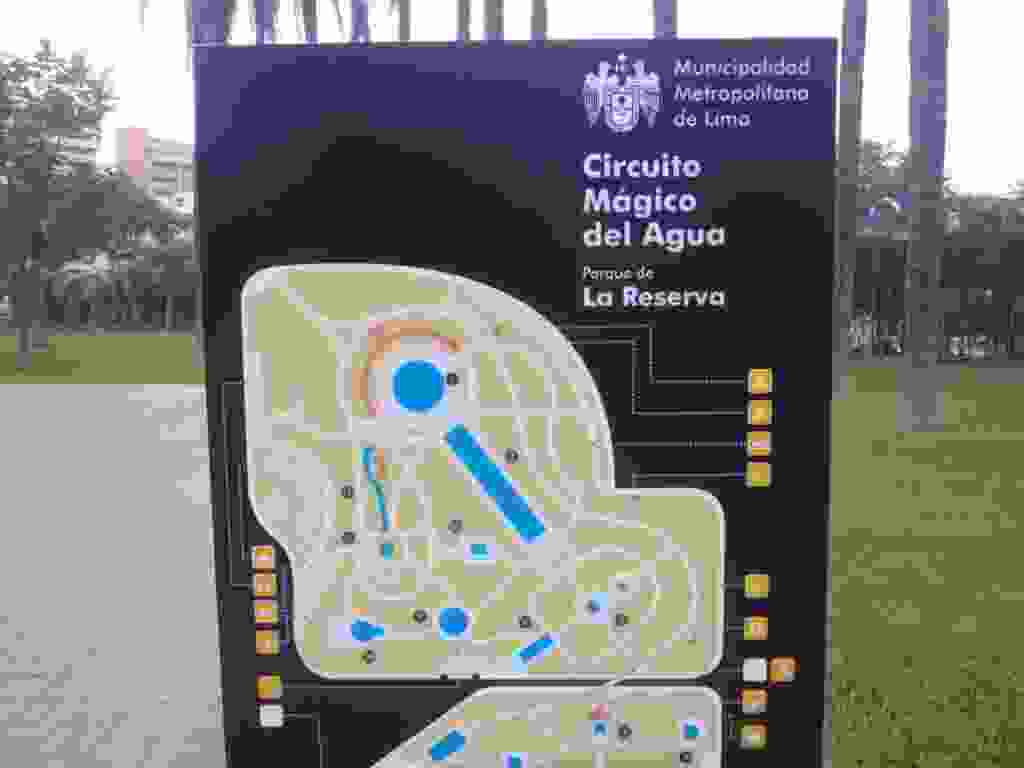
\includegraphics[width=\mywidth]{../wp-content/uploads/2015/06/P6024611-1024x768.jpg} \end{center}

\begin{center} 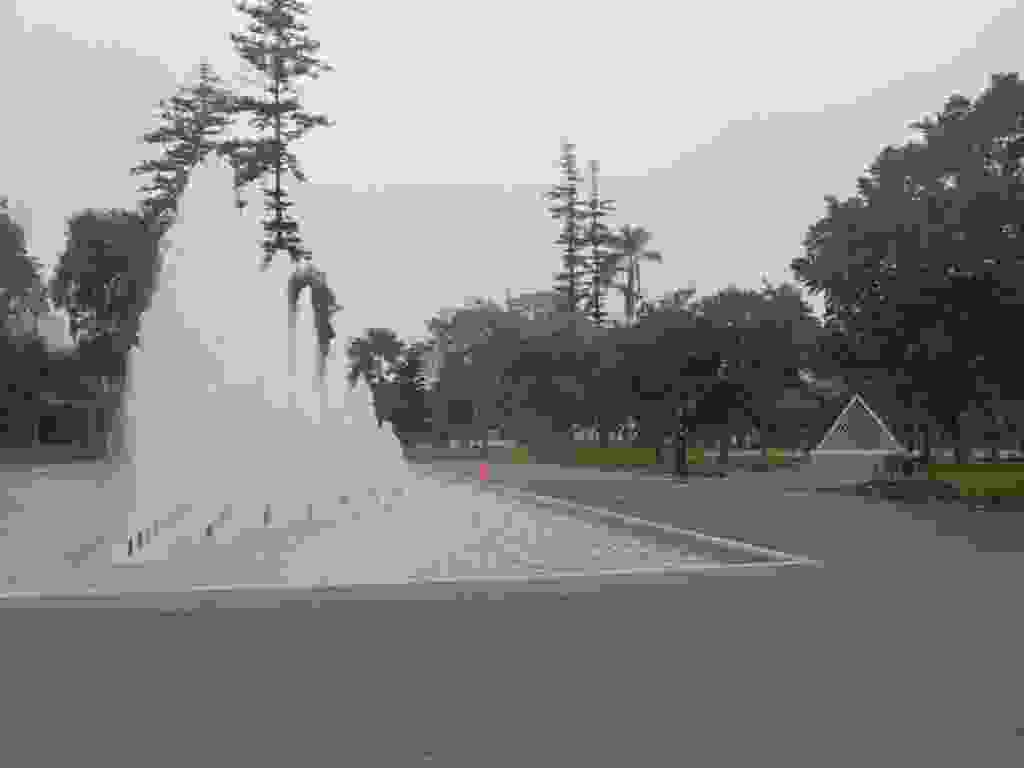
\includegraphics[width=\mywidth]{../wp-content/uploads/2015/06/P6024610-1024x768.jpg} \end{center}

\begin{center} 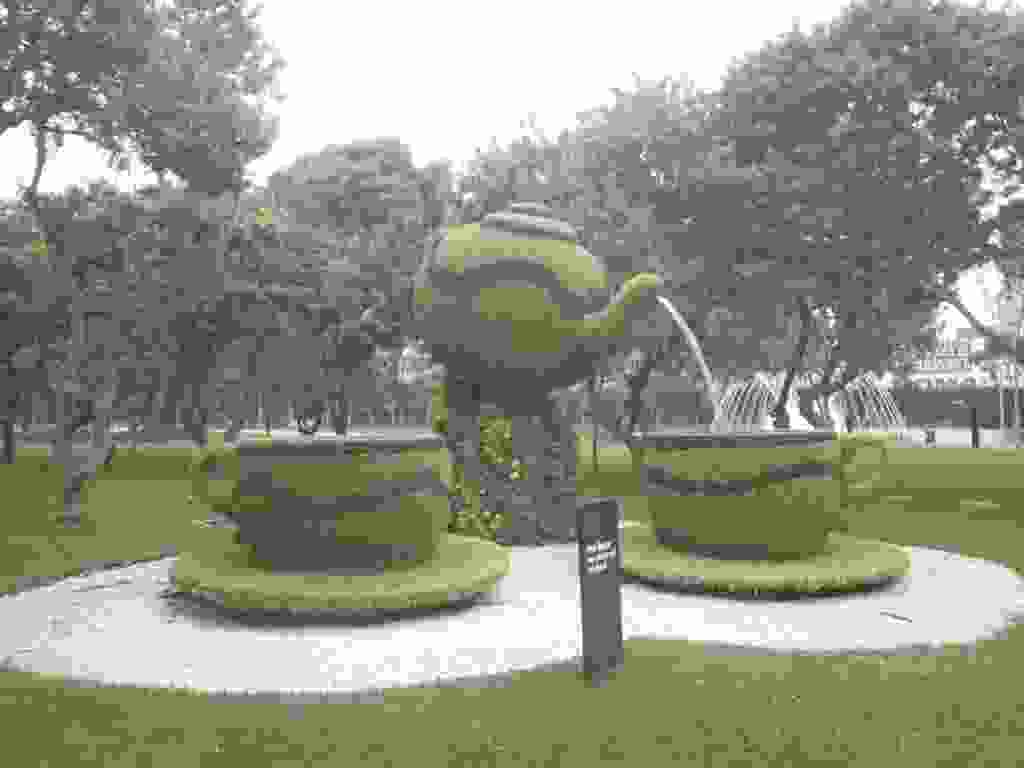
\includegraphics[width=\mywidth]{../wp-content/uploads/2015/06/P6024615-1024x768.jpg} \end{center}

\begin{center} 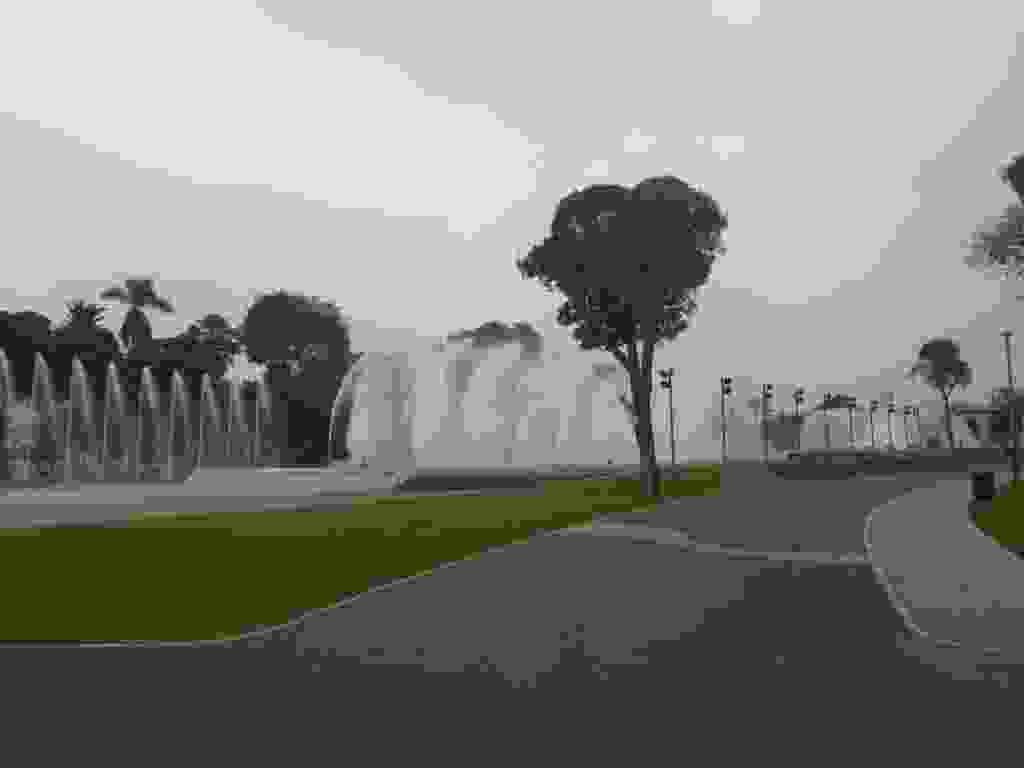
\includegraphics[width=\mywidth]{../wp-content/uploads/2015/06/P6024617-1024x768.jpg} \end{center}

\begin{center} 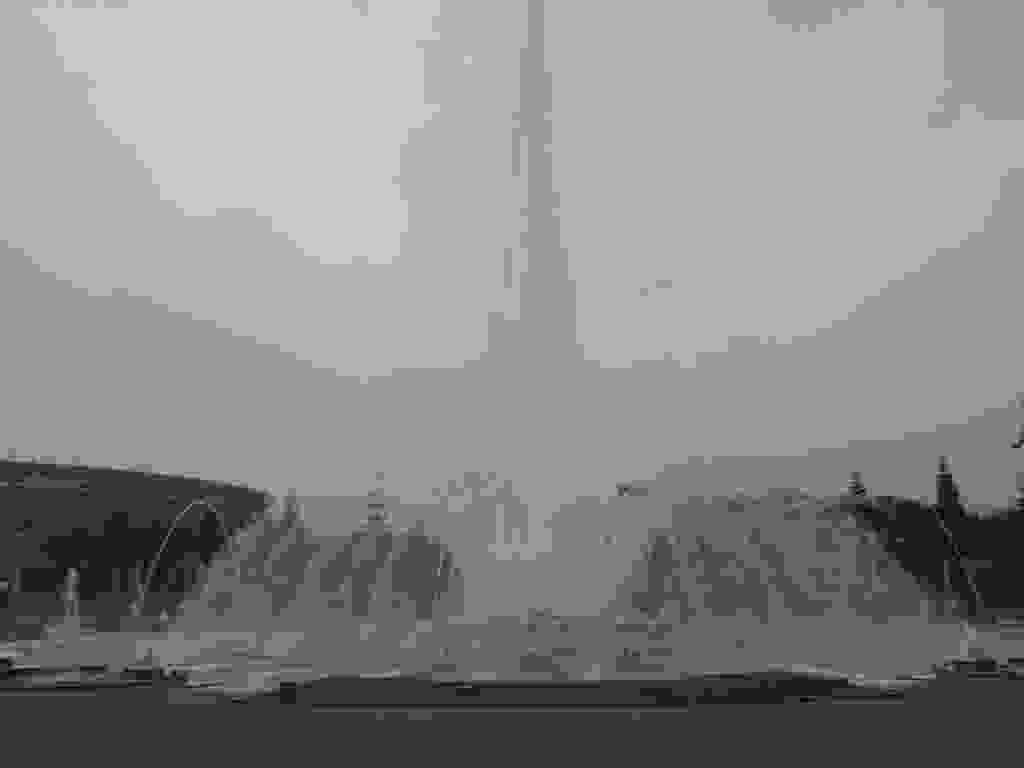
\includegraphics[width=\mywidth]{../wp-content/uploads/2015/06/P6024619-1024x768.jpg} \end{center}

\begin{center} 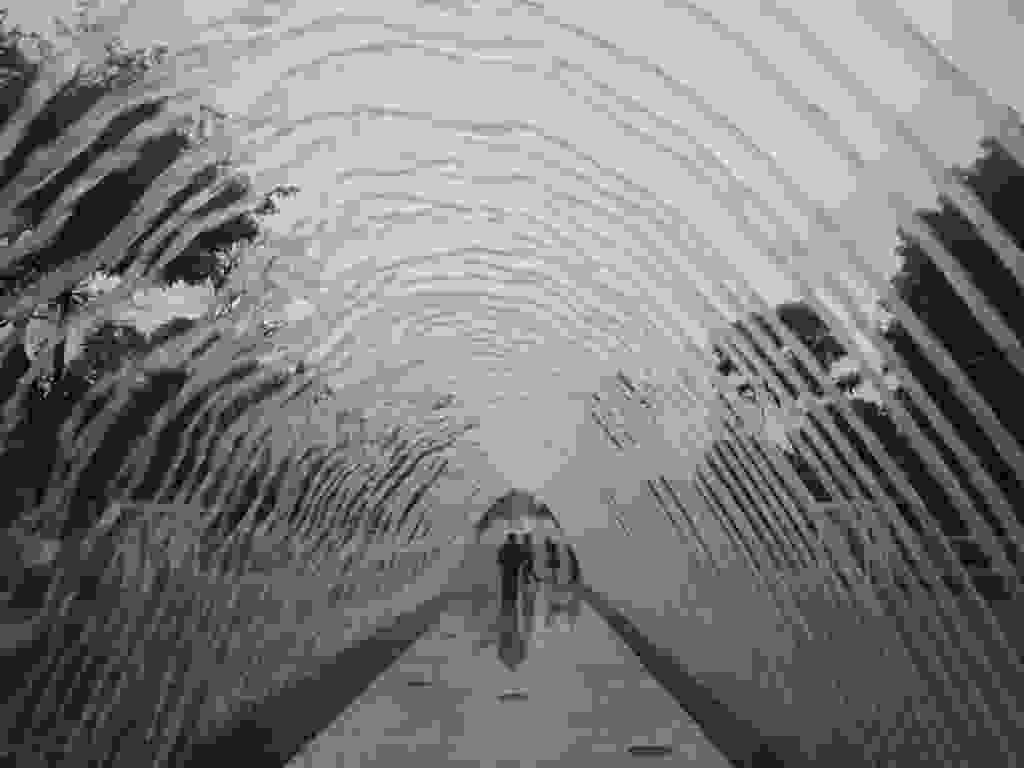
\includegraphics[width=\mywidth]{../wp-content/uploads/2015/06/P6034631-1024x768.jpg} \end{center}